\documentclass[12pt]{article}

\usepackage{enumitem, setspace, graphicx}
\usepackage[margin=1.25in]{geometry}

\setlistdepth{6}

\newlist{packed_enum}{enumerate}{6}
\setlist[packed_enum]{label*=\textbf{\arabic*.},leftmargin=*}

\begin{document}
	\title{Find-Aid: A Bluetooth Sticker Locator}
	\author{Adam Howard \\
		\texttt{ahowar31@vols.utk.edu}
		\and
		Maurice Marx \\
		\texttt{mmarx@vols.utk.edu}
		\and
		John Reynolds \\
		\texttt{jreyno40@vols.utk.edu}
		\and
		Jeremy Rogers \\
		\texttt{jroger44@vols.utk.edu}
		\and
		Matthew Seals \\
		\texttt{mseals1@vols.utk.edu}
		}
	\date{November 2014}
	
	\maketitle
	\pagebreak
	
	\renewcommand{\abstractname}{Executive Summary}
	
	\doublespacing
	
	\begin{abstract}
		A product was requested which would allow the customer to tag an object, specifically a disc golf disc, and then locate the object in the event of misplacing it via a smart device application. In addition to personal consumer use, such a device has applications within the commercial sector for inventory management and location. Because of the intent of using this device for disc golf, extreme requirements were placed on the size and weight of the device, as these factors would affect the flight characteristics of the disc to which the device was attached. The device also needed to have a sufficient communication range with the user’s smart device such that it could be located from across a course, or approximately one hundred meters, and should be priced such that the device would not cost more than the disc it was being attached to. The device should also have enough of a battery life to make it through an afternoon of disc golf without requiring a recharge.
		While the device itself has not been built and prototyped, a reasonable solution to all of the above requirements was found and would likely be feasible given the team’s knowledge of the subject area and skills. A Bluetooth module was discovered that implemented most of the communication stack and which boasted a 100 meter communications range. This was paired with the Bluetooth APIs for Android and iOS, which both have functions for assessing relative distance from a signal source by measuring that signal’s intensity on the smart device’s antenna. A design for the device package was worked out which would provide the system some protection from the elements, and from the shock of impact after being thrown, and affordable rechargeable batteries were sourced which would provide approximately ten hours of battery life while only adding a gram of weight to the package. A method for attaching the device was worked out which would use a double-sided adhesive pad, which would be disposable and enable the consumer to reuse the device with multiple objects.
		Designing for size was by far the most difficult aspect of this project. Fitting within the tight constraints set by the customer forced the Team to make trade-offs in battery life and robustness of the device’s casing, as well as increased the cost for sourcing components. Every gram of weight added by a component hurt, so only what was absolutely necessary to the device’s operation was used. The final part list represents the minimal components which will allow for the devices advertised feature set, while maintaining a minimal impact on the disc’s flight characteristic and the price of materials.
		
		\pagebreak
		
	\end{abstract}
	
		\section{Requirements}
	
		  \vspace{16 pt}
		  
		  \begin{packed_enum}
		  	\item \textbf{Device}
		  	\begin{packed_enum}
		  		\item \textbf{Physical Design}
		  		\begin{packed_enum}
		  			\item \textbf{Package Body}
		  			\begin{packed_enum}
						\item Made of plastic of other lightweight material
						\item Body must cause as little signal attenuation as possible
						\item Body will be water resistant and protect device from the elements
						\item Ideal package weight is 1-3 grams
						\item Package will not interfere with normal usage of target when properly attached.
						\begin{packed_enum}
							\item Aerodynamics of Disc (intended target) must be minimally affected. 
							\end{packed_enum}
		  				\end{packed_enum}
		  				
		  			\item \textbf{Package Interface}
		  			\begin{packed_enum}
		  				\item Access port which enables the user to charge the device's battery charging.
		  				\item \textbf{Button}
		  				\begin{packed_enum}
		  					\item Preferably conductive pad to minimize risk of accidental triggering from environment.
		  					\item Allows user to turn the device on and off
		  					\item Can facilitate registration of device with the application if needed via alternate press method (double-press, long-press, etc.)
		  					\end{packed_enum}
		  				\item \textbf{Status LED}
		  				\begin{packed_enum}
		  					\item Capable of relaying the following device state information to the user.
		  					\begin{packed_enum}
		  						\item Device is powered off.
		  						\item Device is powered on.
		  						\item Device is low on battery power.
		  						\item Device has some internal error.
		  						\item Device is communicating with application.
		  						\item Device has successfully registered with application.
		  						\end{packed_enum}
		  					\end{packed_enum}
		  				\end{packed_enum}
		  			\item \textbf{Adhesive Pad}
		  			\begin{packed_enum}
		  				\item Double-sided pad attached to both device and target.
		  				\item Must be easily removable from both device and target.
		  				\item Minimal residue left of device and target after removal of pad
		  				\item Pad will be made of disposable materials
		  				\item Several pads will be packaged with each device and/or made available separately
		  				\end{packed_enum}
		  		\end{packed_enum}
		  		\item \textbf{Software Specifications}
		  		\begin{packed_enum}
		  			\item \textbf{Modes of Operation}
		  			\begin{packed_enum}
		  				\item While in range of user and communicating with application
		  				\begin{packed_enum}
		  					\item Will remain powered on and active, responding as necessary to input from the application
		  					\item Will indicate that it is in this mode on the status LED defined in (1.1.2.3.1.5)
		  					\item Will periodically wake from low power mode to perform the following actions
		  					\begin{packed_enum}
		  						\item Broadcast a ping containing its MAC address which the application will listen for.
		  						\item Listen for responses to its ping from the application to transition from the current state to that described in (1.2.1.1)
		  						\end{packed_enum}
		  					\end{packed_enum}
		  				\end{packed_enum}
		  			\item \textbf{State Monitoring}
		  			\begin{packed_enum}
		  				\item Device will be able to estimate its total remaining battery life, and reduce the frequency of wake cycles while in the mode described in (1.2.1.2.1) to compensate for lack of power.
		  				\end{packed_enum}
		  		\end{packed_enum}
		  		\item \textbf{Hardware Specifications}
		  		\begin{packed_enum}
		  			\item \textbf{Bluetooth Module}
		  			\begin{packed_enum}
		  				\item Will be self contained and easily programmable.
		  				\item Will not require a separate antenna.
		  				\item Will have an effective range of at least 50 meters in environments with minimal interference.
		  				\item Will be able to sleep and wake periodically as described in (1.2.1.2.1).
		  				\end{packed_enum}
		  			\item \textbf{Speaker}
		  			\begin{packed_enum}
		  				\item Will generate a tone which is clearly audible from around 10 meters away.
		  				\item Will be controlled by the Bluetooth module's processor.
		  				\end{packed_enum}
		  			\item \textbf{Battery}
		  			\begin{packed_enum}
		  				\item Will be rechargeable.
		  				\item Will power the device for several hours while operating in the active state described in (1.2.1.1).
		  				\item Will be charged via the port described in (1.1.2.1).
		  				\end{packed_enum}
		  		\end{packed_enum}
		  		\item \textbf{Tolerances}
		  		\begin{packed_enum}
		  			\item Device will operate within any environment typical of a temperate or moderate climate.
		  			\item Device will be water-resistant if not water-proof.
		  			\item Device adhesive will remain effective in typical environments when attached to smooth, firm surfaces.
		  			\item Device will be resilient to physical shock and impact.
		  			\end{packed_enum}
		  	\end{packed_enum}
		  	\item \textbf{Application}
		  	\begin{packed_enum}
		  		\item \textbf{User Interface}
		  		\begin{packed_enum}
		  			\item \textbf{Device Registration View}		  			\begin{packed_enum}
		  				\item Will show a list of all devices registered with the application.
		  				\item Devices will have a user-customizable identifier.
		  				\item Will show devices which are unregistered but within communications range of the device upon which the application is running.
		  				\item Will allow the user to add unregistered devices to the registered list. 
		  				\end{packed_enum}
		  			\item \textbf{Device Location View} 
		  			\begin{packed_enum}
						\item Will be associated with a specific device.
						\item Will show that device's identifier somewhere on the screen.
						\item Will use a meter to visualize the detected signal strength of the device currently in focus.
						\item Once within communications range, a button will appear within the view to allow the user to toggle the speaker on the device which is currently in focus.
		  				\end{packed_enum}
		  		\end{packed_enum}
		  		\item \textbf{Device Communications}
		  		\begin{packed_enum}
		  			\item \textbf{One-way Communications}
		  			\begin{packed_enum}
		  				\item Application will periodically ping the device to see if it has come into range.
		  				\item Application will listen for the device's pings to discern location based on signal strength.
		  				\end{packed_enum}
		  			\item \textbf{Two-way Communications}
		  			\begin{packed_enum}
		  				\item Application will send a confirmation signal to the device once it has been successfully registered.
		  				\item Application will periodically ping the device to discern it it is still within range.
		  				\item Application will send a toggle signla whenever the user presses the speaker toggle button.
		  				\end{packed_enum}
		  			\item \textbf{Out of Range}
		  			\begin{packed_enum}
		  				\item After a timeout period has elapsed the application will mark a registered device as ``out of range''.
		  				\item If a ping is received from a registered device marked ``out of range,'' it will be marked as ``in range'', and its signal strength should be made available to the user to view.
		  				\end{packed_enum}
		  		\end{packed_enum}
		  		\item \textbf{Platform Compatibility}
		  		\begin{packed_enum}
		  			\item Will be available for any Bluetooth-enabled Android or iOS device through the Google Play Store and the App Store.
		  			\end{packed_enum}
		  		
		  	\end{packed_enum}
		  \end{packed_enum}
	
	\section{Design Process}
	\subsection{Device}
	The design process used was both efficient and effective. After analyzing the requirements document, the team worked through the document by focusing on a single point at a time. A decision was made for each point before proceeding. When a requirement called for specific technology or consistency, potential solutions were researched heavily. The final product and its underlying components were agreed upon only once all of the headers and sub-headers of the requirements document had been addressed. This section of the paper details in-depth the process of building the Find-Aid product from the ground up.

Beginning with the \emph{Device} and its \emph{Physical Design/Package} Body sub-headers, the team decided that a plastic or rubberized plastic material would fulfill all of the requirements. A plastic or rubberized plastic has many desirable properties: it is water resistant, lightweight, and can be molded for optimal aerodynamic performance. Further, it causes minimal signal attenuation. The size of the plastic housing can be tailored to fit all of the required components while also maintaining a weight between 1 and 3 grams. It is also easily cut, allowing for easy placement of a Micro USB port, which will be used to recharge the lithium-ion battery. 


The \emph{Physical Design/Package Interface} was analyzed second. Its design supports three features. The package’s interface provides two mediums for important user interactivity. Users are able to charge the device’s lithium ion battery by connecting it to a power source via a port located on the device body, and users are able to turn the device off and on with a power button. The power button may also double as a bluetooth pairing function facilitator, meaning it can be used to connect the device to a nearby user’s application. Lastly, an LED light representing differing states of the device will be located on the exterior of the device housing, and it will be powered by the internal lithium ion battery.


The \emph{Physical Design/Adhesive Pad} refers to the product that attaches the Bluetooth locator sticker to the target device. The pad is required to have a strong adhesive that could withstand shock from everyday use, as well as be able to operate in wet environments resulting from inclement weather. The adhesive pad is required to be water resistant, but not completely waterproof. Rather than design our own adhesive pad, we chose to consider commercially available products that would meet the requirements specified. A good candidate was the Command™ brand strips, which are available in many retail stores. They are rugged and inexpensive, which would allow us to package many of them with our product. Removal of the strips also leaves no residue on the target device or the Bluetooth locator.


Two of the categories found in the product requirements are directly related: the \emph{Software Specifications} header (1.2) and the \emph{Bluetooth Module} sub-header (found under the \emph{Hardware Specifications} header; 1.3.1). The software capabilities depend upon the hardware capabilities. Thus, the two have been evaluated simultaneously. However, in order to retain a coherent flow in this paper, the pair will be described separately, and the \emph{Bluetooth Module} will not be described until it is appropriate (considering chronological order). 


The \emph{Software Specifications} in section 1.2 can be met exactly as requested because of the Bluetooth module chosen. Hardware can be connected to directly in order to control data flow in the Bluetooth module. The software will remain powered when in range of the user and engaging in communication. It will be connected to the LED status indicator on the exterior of the device housing, and will be constantly updating its color (as per 1.1.2.3.1.5). The Bluetooth MAC address will be broadcasted periodically. This provides pairing capabilities to nearby applications. When a user’s application signals the Bluetooth device requesting the buzzing feature be activate, the software will facilitate this activation. If the user’s application surpasses the Bluetooth module’s maximum distance, the device will go into “sleep” mode. While in this mode, the device will periodically broadcast its MAC address. If the ping is rebounded by the user’s application, the device will awaken from sleep mode and return to full power. The on-board software is also responsible for the monitoring of remaining battery life. The frequency of wake cycles will be altered depending on remaining power (1.2.2.1).


The \emph{Hardware Specifications/Bluetooth Module} is an integral component of the device. Many Bluetooth capable components exist. However, the RN4020 Bluetooth module provides all of the functionality necessary for adherence to the requirements specification. The module is 11.5 x 19.5 x 2.5 mm in size, which makes it plenty small enough to fit in the device housing. It  has a completely configurable software stack and good power consumption rates. The MAC address is accessible and all data transmission can be encrypted. The RN4020 module provides the basis of functionality for the entire product.

The \emph{Hardware Specifications/Speaker} and \emph{Hardware Specifications/Battery} will be connected. The battery, RN4020, and the RGB LED will all be connected by a circuit allowing recharging through a Micro USB port. The RN4020 has pins allowing for direct connection to the buzzer and RGB LED, so that the Bluetooth module may control the color the LED emits as well as signal the piezoelectric buzzer to activate. With all of these component combined, the functionality of the device is now complete.


\emph{Hardware Specifications/Tolerances} requirements are important to the reliability of our final product. The device must reliably work within reasonable climate and environment changes. The device may be made water-resistant with the use of rubberized plastic housing. Further, a cap may be created that fits into the  recharging port effectively keeping water out. The adhesive chosen is both effective and disposable, and has good resistance to changing environmental temperature. Lastly, because the device housing is made of a plastic (or rubberized plastic), it is resilient to moderate physical impact. This should provide more than enough tolerance for the given problem: disc golf.


The above design analysis applies specifically to the device. With all components combined, the final product will meet all requirements specifications. The user Application is provided with full functionality. All hardware features requested have been met, and the hardware analysis provides a scaffolding for the Application design analysis. A mockup of what the device would look like is shown in \textbf{Figure 1}. Because of the Bluetooth module chosen, the application can easily connect to and request service from a given paired device. All that must be implemented on the Application is the interface for intercommunication between the smartphone application and the bluetooth module that is located inside of the device. The application’s design will now be analyzed.

\begin{figure}
	\centering
	\caption[Figure 1]{}
	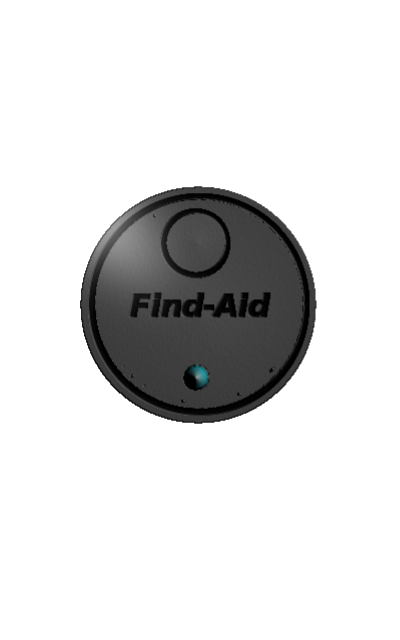
\includegraphics[width=.33\linewidth, height=.4\textheight]{/Users/jroger44/Downloads/find}
	\label{fig:find}
\end{figure}

		\subsection{Application}
		The design process of the application adhered very closely to the requirements specifications given. The \emph{User Interface} was looked at first, and the rest of the requirements were iterated through systematically.
		
		We first looked at the two views that we were required to create, the \emph{Device Registration View} and the \emph{Device Location View}. \textbf{Figure 2} shows the first part of the Device Registration View. As one can see from the image, it shows a list of all devices registered from the application, and each registered device has its own user-customizable identifier.
		
\begin{figure}
\centering
\caption[Figure 2]{}
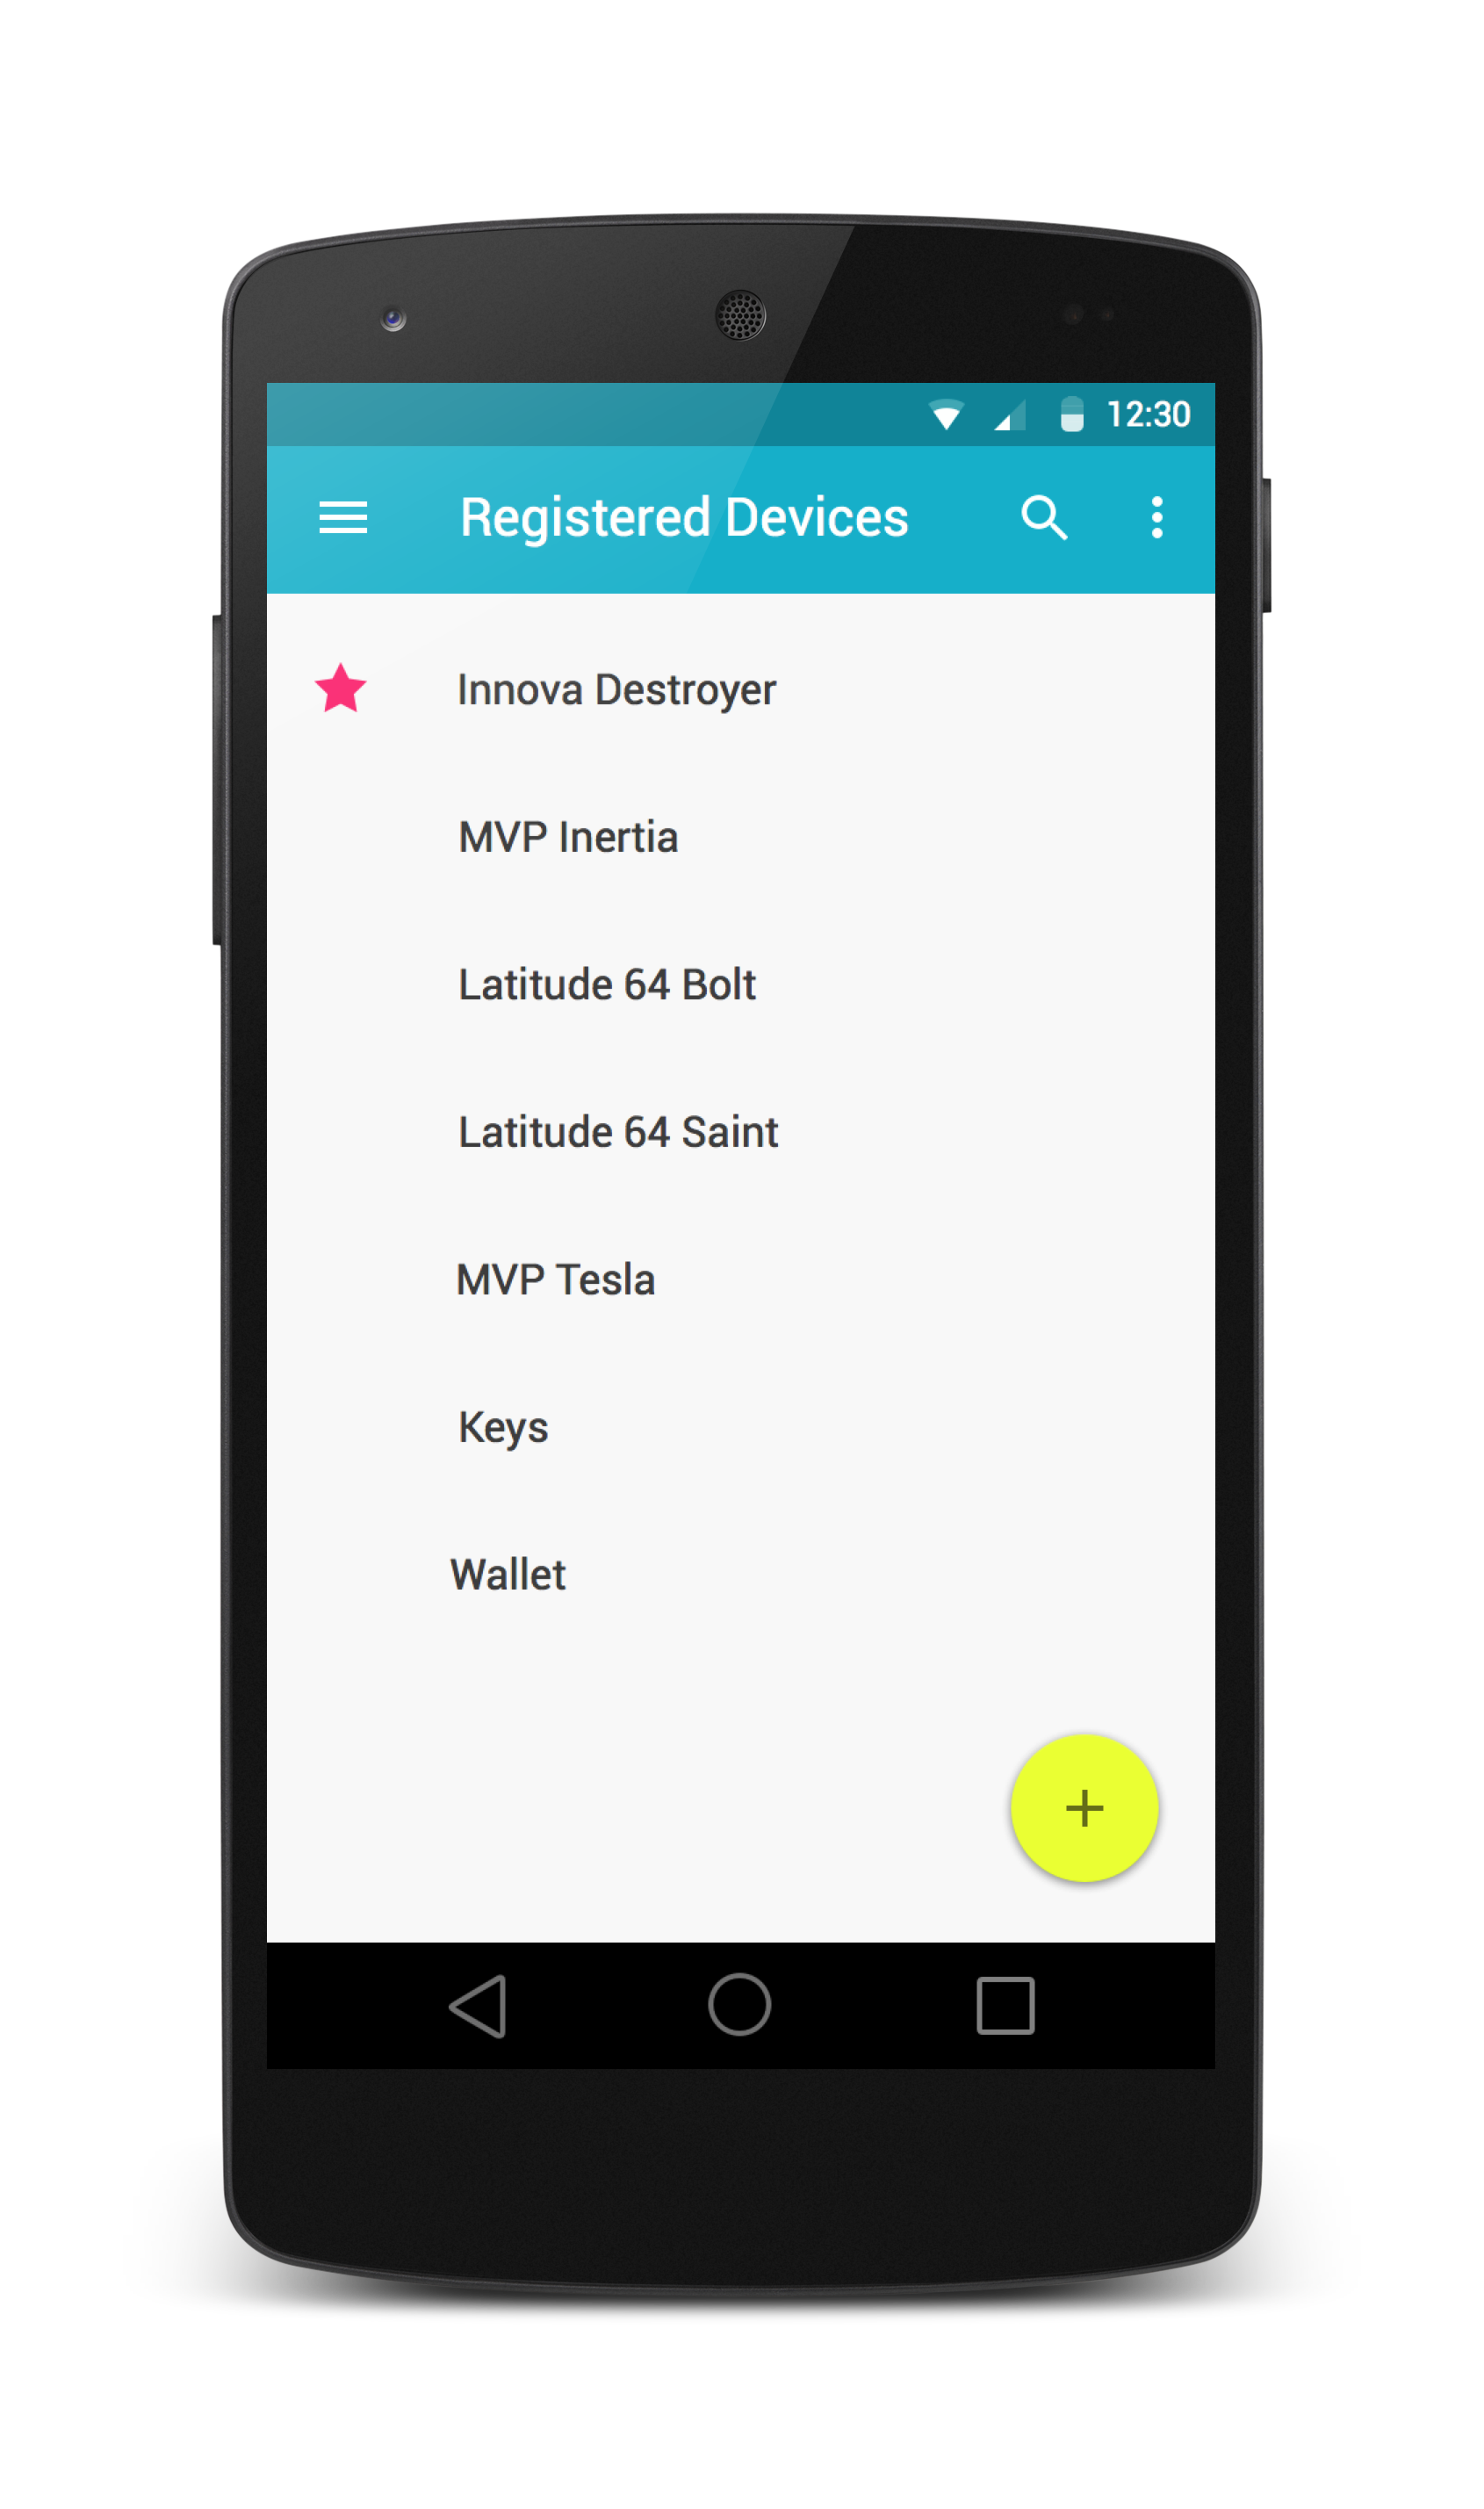
\includegraphics[width=.33\linewidth, height=.4\textheight]{/Users/jroger44/Downloads/Devices_framed}
\label{fig:Devices_framed}
\end{figure}

		The second part of the Device Registration View is shown in \textbf{Figure 3}. In this part of the view, it shows the Bluetooth MAC addresses of the devices nearby that are unregistered but within communications range of the device using the application. The user can then give the unregistered device an identifier and add it to the list of known devices.
		
\begin{figure}
\centering
\caption[Figure 3]{}
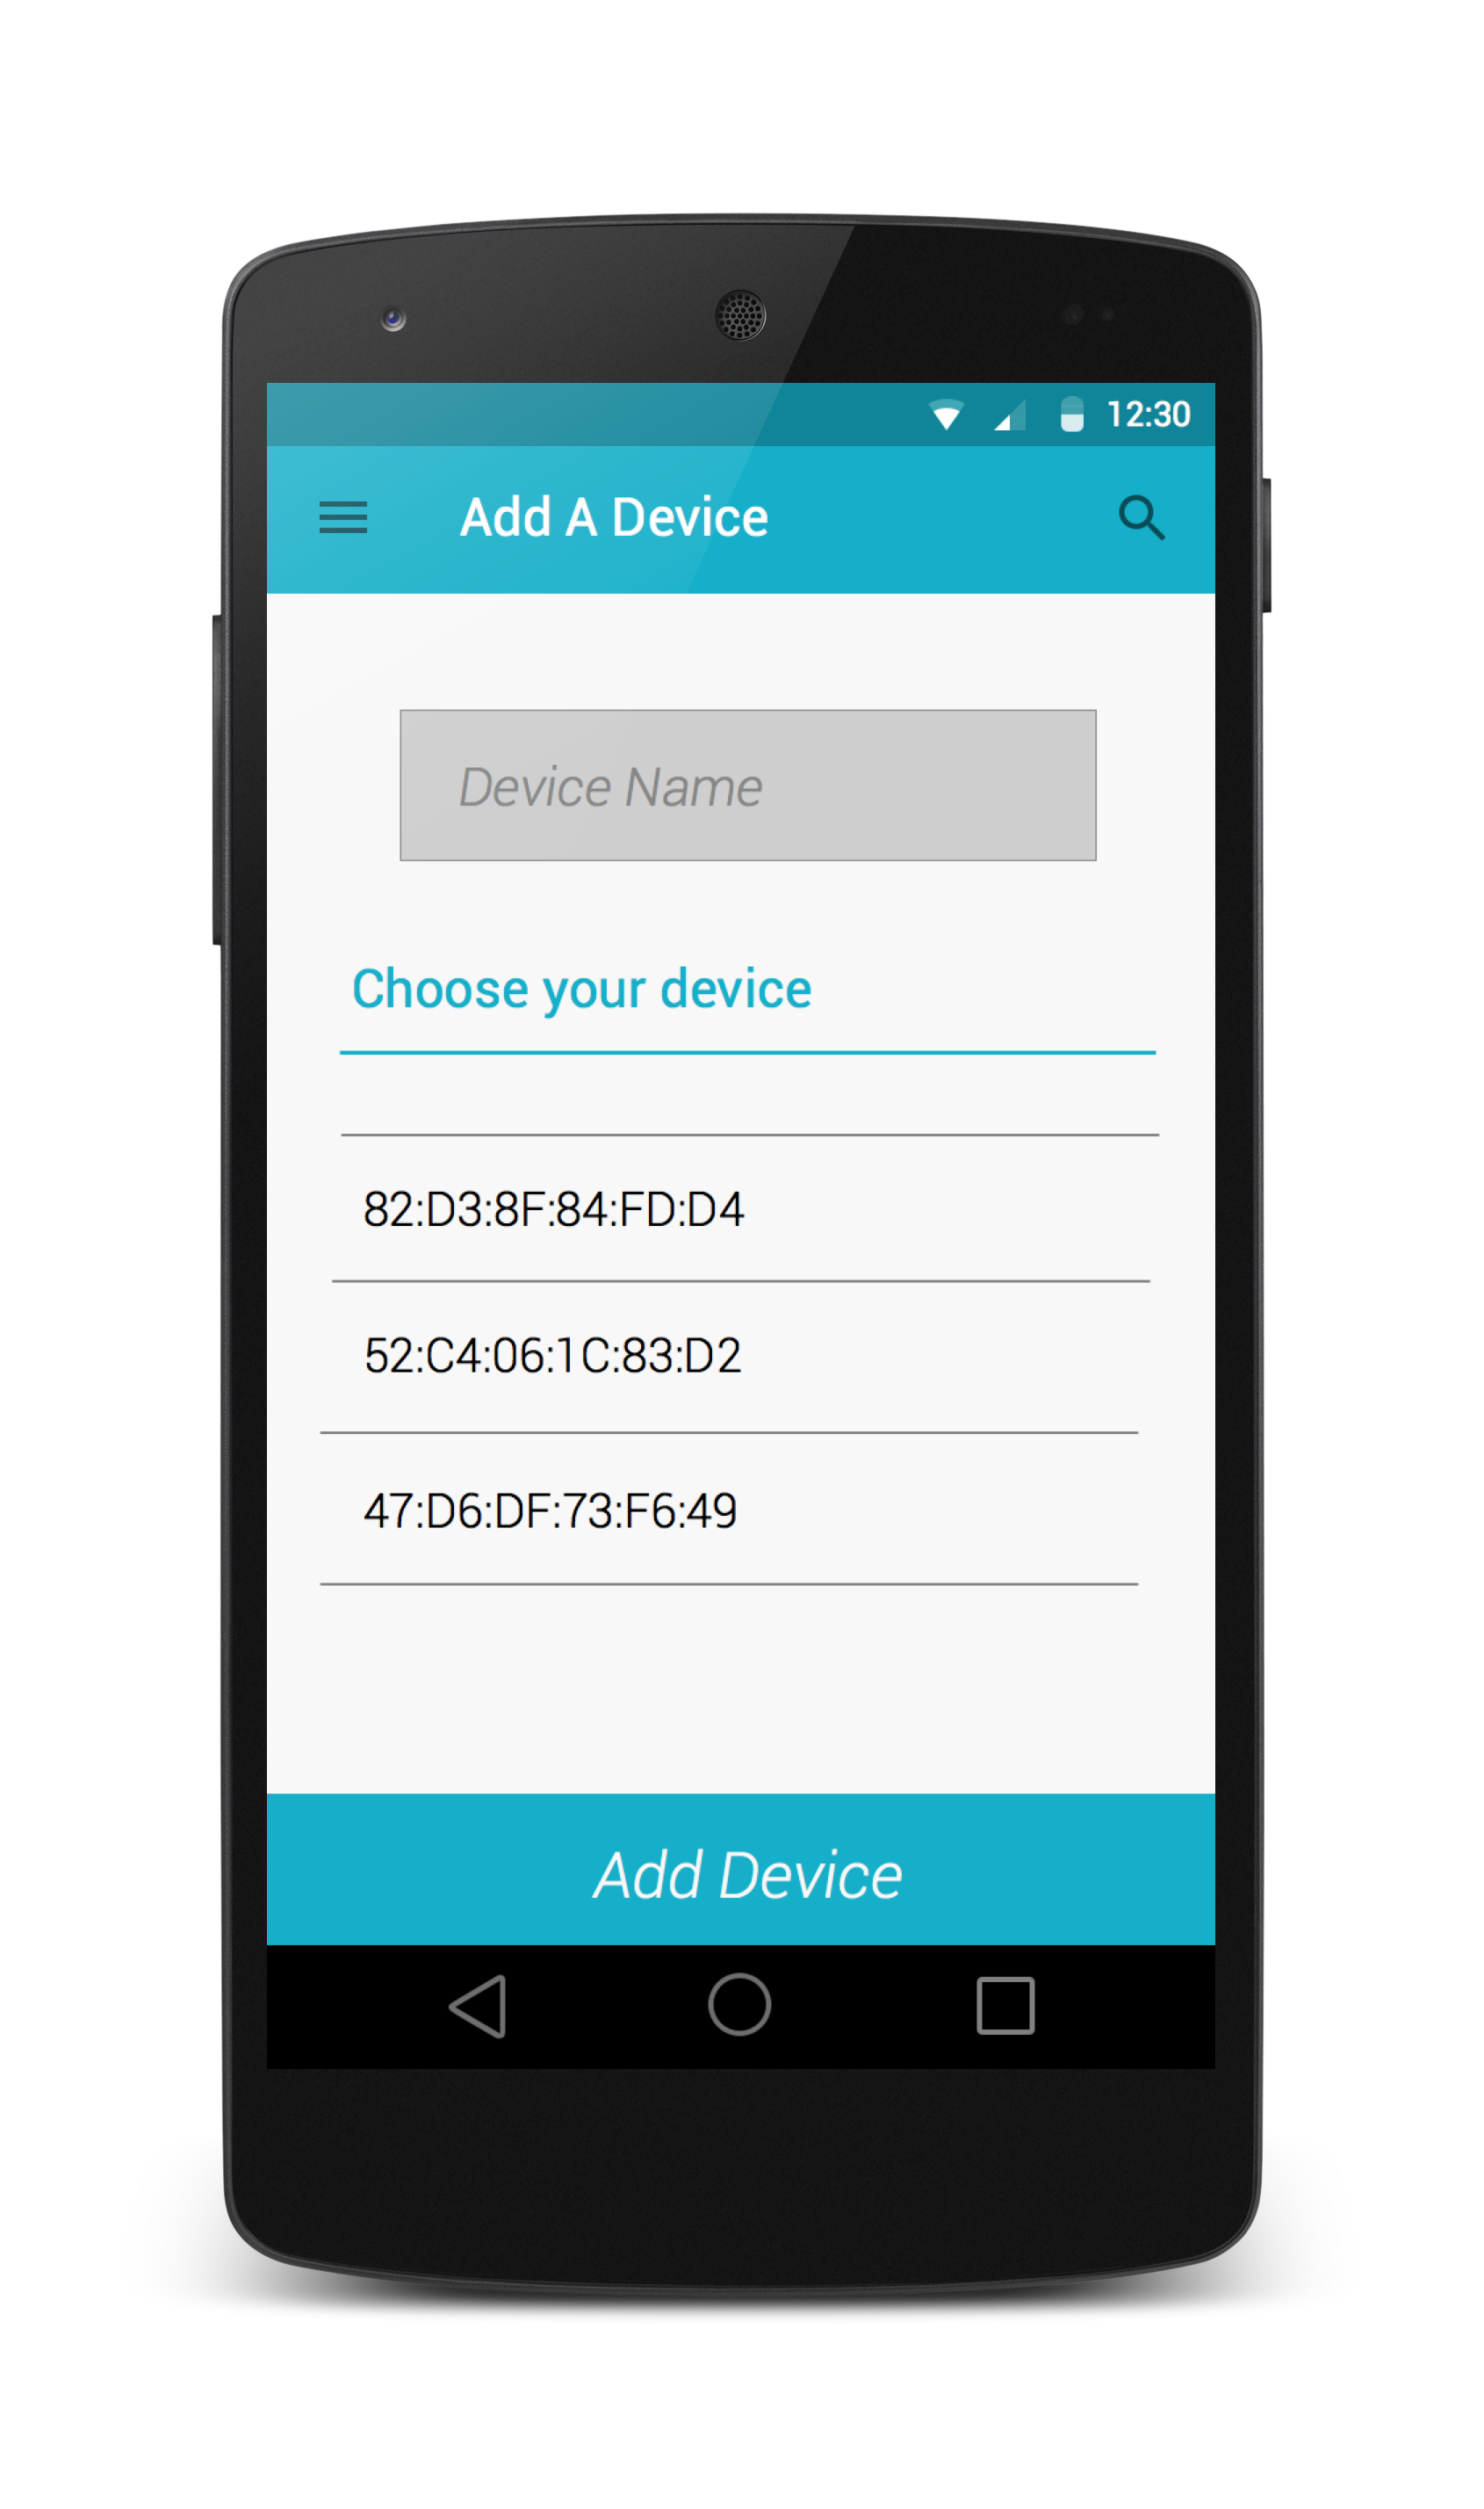
\includegraphics[width=.33\linewidth,
height=.4\textheight]{/Users/jroger44/Downloads/AddDevice_framed}
\label{fig:AddDevice_Framed}
\end{figure}

		The next part of the application design process is the \emph{Device Location View}. Each view is associated with a specific device, and that device's unique identifier is shown on the screen. There is a meter to visualize the detected signal strength, via RSSI. The ``buzzer'' button will be greyed out until the signal strength reaches a certain point. This is shown in \textbf{Figure 4}. The figure shows the identifier given to the device at the top of the screen, and shows the signal strength indicator in the middle of the screen. At the bottom there is the buzzer button that will activate the piezoelectric buzzer on the device. 

\begin{figure}
	\centering
	\caption[Figure 4]{}
	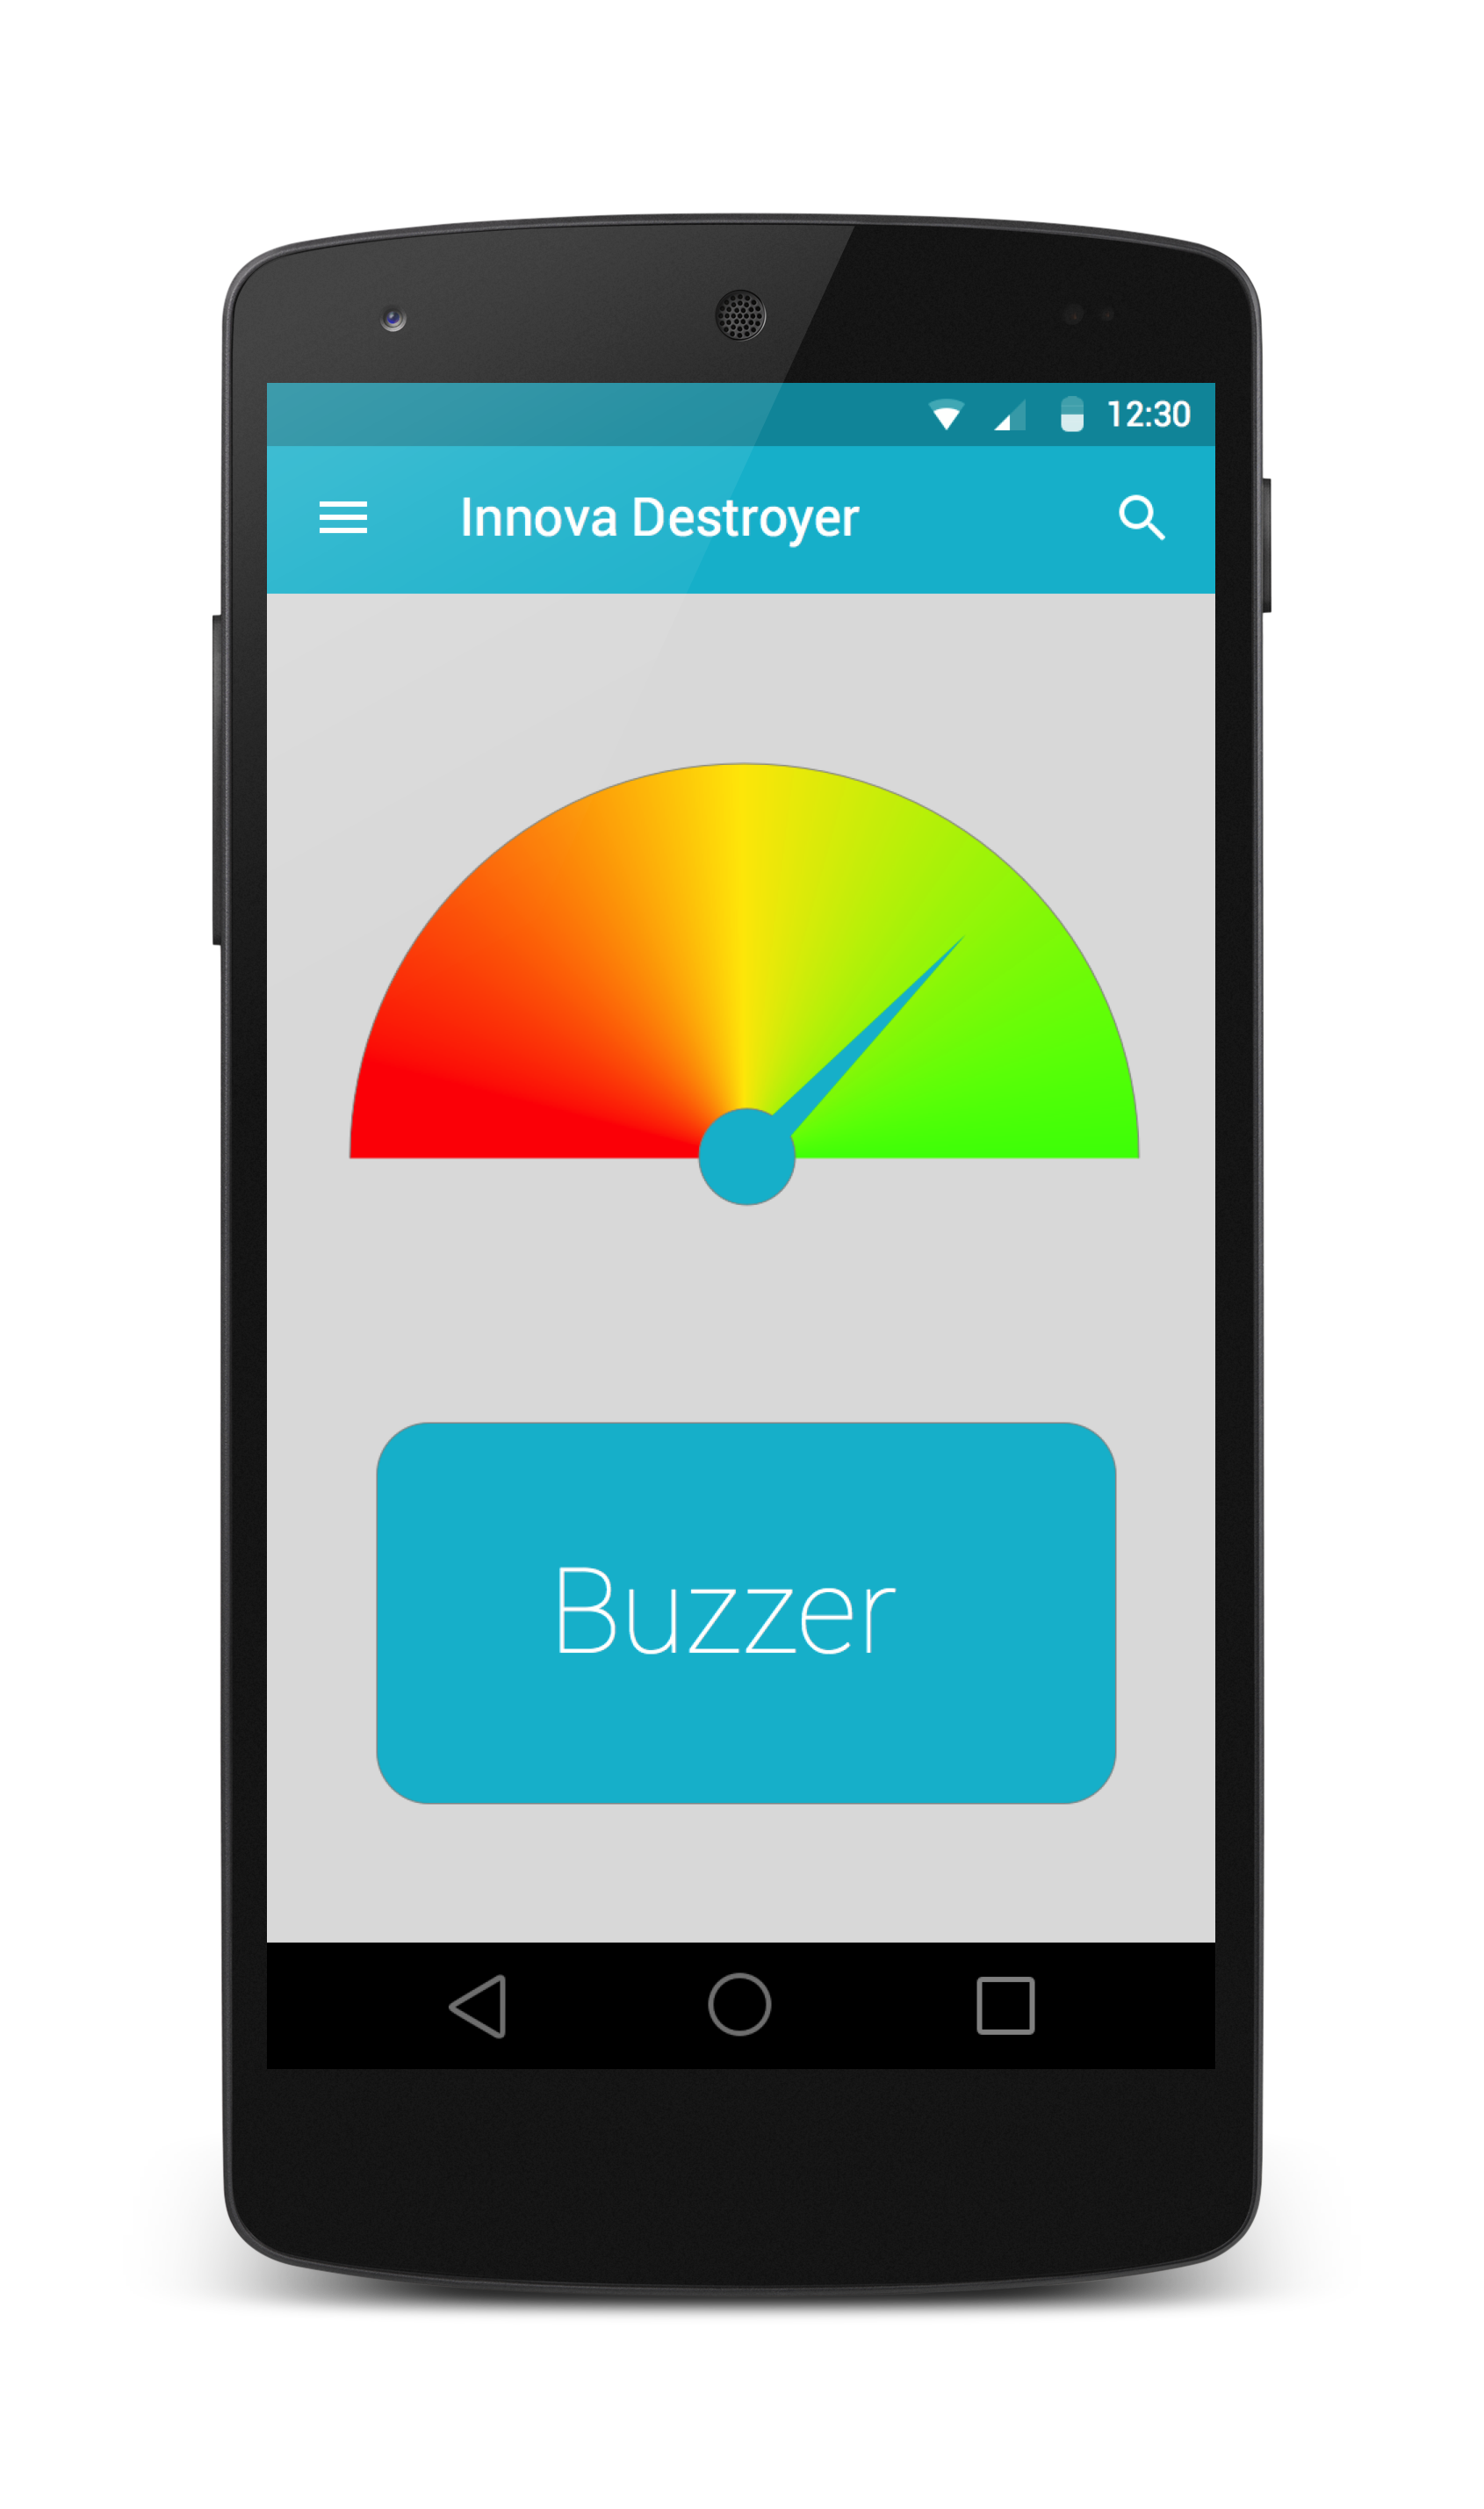
\includegraphics[width=.33\linewidth,
	height=.4\textheight]{/Users/jroger44/Downloads/FindDevice_framed}
	\label{fig:FindDevice_Framed}
\end{figure}

	The application would periodically ping the device to check if the device is in range. It would also listen for pings from the device. Once a device goes out of range, it would list it as such, and wait for the device to come back in range. Once back in range, the application would make the signal strength available to the user. The application would also be distributed on the Google Play Store and the App Store.
	
	\section{Final Results}
	
	This section will describe the results of our semester of work. These results would be written much differently had we actually implemented our product. Since this was not the case, this section will primarily discuss the testing suite. There are two parts of testing: the first part, which discusses things we actually tested, and the second part, which discusses things that we would test if we were actually implementing the product. 
	
	For the first part, we did actually test the change in flight characteristics of each disc. The course of action we took on this was going into a large field and throwing each disc two times, once with no weight, and once with 2 quarters taped to the bottom of each disc. Two quarters is close enough to the size and weight of our device mockup to be substantial testing. When the flight patterns were compared after all of the discs had been thrown twice, the distances were only marginally affected. Some of the discs were actually thrown farther with the added weight than previously. As far as flight patterns go, they were inconsistent at best, but that can be attributed to the inconsistency of the person throwing the disc. 
	
	Secondly, if we were implementing this project in full, we would have many more things to test. First, the testing of the discs that we did would not be substantial enough to call them definite. More extensive testing would be required. To do more testing, we could either get an outside person who is more consistent with throws to test the flight patterns, or we could simply get a machine that would do the throwing for us. However, the largest part of the actual testing would come from testing the hardware. There are many aspects of the hardware that need to be tested. For one, we would need to test the range of the RN4020 Bluetooth module. To do this, we would get multiple smartphones, and try to get on the outermost part of the advertised range of the RN4020, and then slowly move towards the module until we get a signal. This would give us the maximum possible range of our device. To continue testing, we would have to test the waterproofing ability of the rubberized plastic enclosure, preferably before putting the actual design into it. This could be done by simply sticking a water damage indicator sticker on the inside of the enclosure, closing it, and then splashing water on it for a while to see if the paper indicates that water has been inside of it. Another large part of the testing suite would be testing the application software. Most of this would be done incrementally as we would move on with development of the application and would be the type of testing that can't be written about, because we cannot be sure what it is until something does not work.  
	
	\section{Lessons Learned}
	
	As a result of strong communication among team members, we were able to minimize the frequency of unexpected events. We were not completely free from unforeseen contingencies, however. When turning in our first group assignment, we were not explicit about who would be responsible for submitting the final draft. This led to some confusion and resulted in us turning our first assignment in a little late, even though it was finished on time. After this minor hiccup, the team leader was delegated to turn in all final copies of assignments, making sure that the mistake would not be repeated. 
	When first beginning to work together, there were times when the delegation of tasks to individual team members was not clear. This was very short-lived, however, and our team quickly improved our communication to make sure that we always knew exactly what we were responsible for. The poor communication early on in the semester can partially be attributed to a lack of familiarity among team members, which was quickly overcome. 

	In future projects we would like to use a revision system to organize documents related to our project. It would help track the contributions made by individuals and would prevent work on multiple copies of the same document. Currently, we share our work via attachments in emails that are forwarded to everyone in the group. Using the most up to date document can be confusing when multiple people have contributed to the same piece of writing and emailed their revision to the group. In our group, there is one team member who is responsible for collecting the fragments of each document and piecing them all together to create the final version of an assignment. A document revision system would greatly aid this individual, because he could directly translate one document to its final format, rather than having to look through emails to piece the final version together. 	
	
	\section{Individual Contributions}
	
	    As team lead, it was my responsibility to see that everyone on the team knew what they needed to do, and when they needed to do it. I was responsible for scheduling meetings, being our spokesperson with Dr. Birdwell, and communicating with the customer. I was also responsible for ensuring that deliverables were submitted on time, and coordinating my team members’ skills and knowledge to ensure that they were best utilized. 
	    
	    As one of the primary researchers, and the only member of the team really comfortable with circuit design, it was also my responsibility to research devices and solutions that would work for our particular application. This included researching parts and trying to ensure that every part picked fit within the stringent weight limits of the design problem. As a part of this role, I was responsible for a significant portion of the requirements document and the final device design.
	    
	    \emph{-Adam Howard,
	    	 Team Lead,
	    	 Librarian,
	    	 Researcher,
	    	 Writer} \\
	    
	    My main contributions to the project entailed writing sections of the different written reports which were assigned to us. Specifically, I played a minor role in the writing of the ``Needs \& Requirements Specification,'' and a larger role in the writing of the "Analysis and Solution Strategy." More recently, I contributed to the final report by detailing the design process of our mobile application, which is the counterpart to our Bluetooth device sticker. Having an active and consistent role in the documentation of our project allowed me to progressively observe the evolution of our project throughout the semester.
		
		\emph{-Maurice Marx,
			Lead Writer,
			Designer,
			Researcher} \\
		
		I made many contributions to this team project. I worked on the design of the device. I personally made both the "Need/Concept/Market/Competition" Powerpoint presentation and the "Design Analysis" presentation, which means that I was responsible for both of the presentations our group had to give in class. Further, I helped to write the "Analysis \& Solution Strategy Report” and the final report.
		
		\emph{-John Reynolds,
			Designer/Implementer,
			Tester} \\
		
		As the Solutions Architect, my main job was to come up with effective solutions to the team that we could use in the project. This was relatively easy for me since I have been a disc golf enthusiast for a few years. This allowed me to come up with how the discs would fly differently based on what shape, size, and weight object we put on them. I also have a superfluity of first hand experience with losing discs, so that experience was helpful in coming up with ideas for the project. Another one of my roles was the Lead Presenter role. John made the powerpoints, which means that I was responsible for making sure that each slide was accounted for, and that everyone could give informed presentations on each topic. My last role as a writer was to compile each member's contributions to each paper into one document. Since I was the only person in the group to be fluid in \LaTeX, I was assigned this role. 
		
		\emph{-Jeremy Rogers,
			Solutions Architect,
			Lead Presenter,
			Tester,
			Writer} \\
		
		My main contribution to the project was making the poster. I took on this role since I already had previous experience in making a poster over the summer at Oak Ridge National Laboratory for my internship. The ORNL poster went over well, so I knew this one would as well. My other contributions were learning about the features of the device and how it worked as well as the market of this device so I would be able to accurately give my portion of the presentations.
		
		\emph{-Matthew Seals,
			Lead Tester,
			Designer,
			Reviewer}
		
		\pagebreak
		
		
\includegraphics[width=0.4\linewidth]{/Users/jroger44/Downloads/Adamsig}

		\textbf{Adam Howard} \hfill\\
		
		
\includegraphics[width=0.4\linewidth]{/Users/jroger44/Downloads/Mauricesig} \\
		
		\textbf{Maurice Marx} \\
		
		
\includegraphics[width=0.4\linewidth]{/Users/jroger44/Downloads/Johnsig}
		
		\textbf{John Reynolds} \\
		
		
\includegraphics[width=0.3\linewidth]{/Users/jroger44/Downloads/Jeremysig}
		
		\textbf{Jeremy Rogers} \\
		
		
\includegraphics[width=0.3\linewidth]{/Users/jroger44/Downloads/Matthewsig}
		
		\textbf{Matthew Seals} 
		
	
	\end{document}

